\section{Introduction to Operating Systems}

\begin{remark}
    Content:
    \begin{itemize}
        \item Basic Principles of Operating Systems
        \item Computer Hardware Review
    \end{itemize}
\end{remark}

\subsection{Basic Principles of Operating Systems}

\begin{concept}{Operating System (OS)} as an extended machine
    \begin{itemize}
        \item Software that manages computer hardware
        \item Provides services for programs
        \item Acts as intermediary between user and hardware
    \end{itemize}
    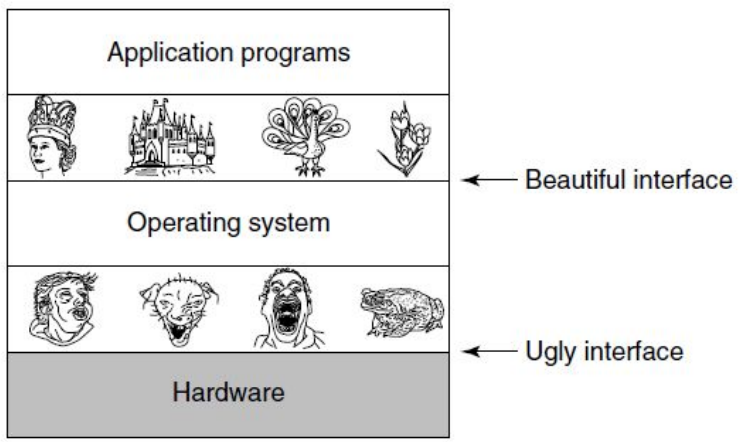
\includegraphics[width=\linewidth]{OS_overview.png}

    Hardware is very complicated: The job of the operating system is to create good abstractions 
    and manage the abstract objects thus created.
\end{concept}

\begin{definition}{Operating System (OS)}
    \begin{itemize}
        \item User Mode vs Kernel Mode
        \item Northbound Interface: User Interface
        \item Southbound Interface: Hardware Interface
    \end{itemize}
    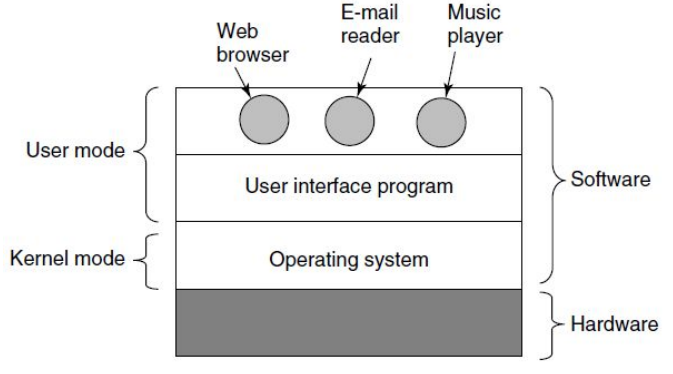
\includegraphics[width=\linewidth]{OS_def.png}
\end{definition}

\begin{concept}{OS as a Resource Manager}
    \begin{itemize}
        \item Process Management
        \item Memory Management
        \item File System Management
        \item Device Management
        \item Security
    \end{itemize}
    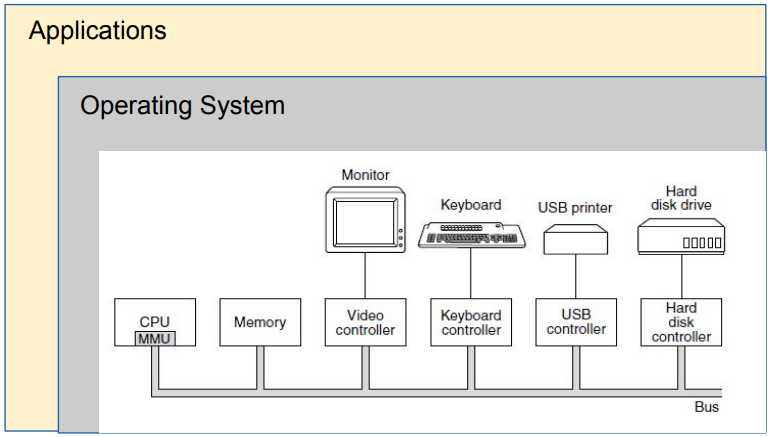
\includegraphics[width=\linewidth]{os_resource_magaer.png}

    The OS controls resource usage, grants resource request, accounts for usage and mediates conflicting requests.
\end{concept}

\subsection{Computer Hardware Review}

\begin{definition}{CPU} Central Processing Unit\\
    \begin{itemize}
        \item Basic cycle: Fetch, Decode, Execute
        \item CPUs feature some registers to hold key variables and temporary results
        \item Special registers for internal use: Program Counter (PC), Stack Pointer (SP), Program Status Word (PSW), etc.
    \end{itemize}
    \vspace{2mm}
    CPUs and their Instruction Sets are architecture-specific:
    \begin{itemize}
        \item ARM, RISC, X86, etc.
        \item Instructions are classified along Execution Privileges, enforced by CPU:
        \begin{itemize}
            \item Intel: User Mode (limited set of instructions) vs Kernel Mode (full set of instructions)
            \item ARM: UnPrivileged Mode vs Privileged Mode
        \end{itemize}
    \end{itemize}
\end{definition}

\begin{concept}{CPU cycles}\\
    Basic cycle of every CPU:    
    \begin{itemize}
        \item Fetches the first instructions from memory into registers
        \item Decodes instructions (determining type and operands)
        \item Executes instructions
        \item fetch, decode, execute, ...
    \end{itemize}
CPUs have multiple cores, each having multiple execution units and parallel pipelines:

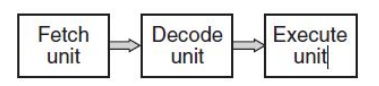
\includegraphics[width=0.6\linewidth]{cpu_cycles1.png}\\
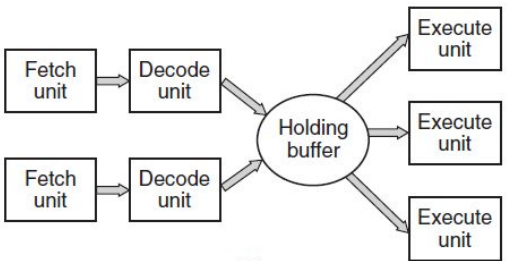
\includegraphics[width=\linewidth]{cpu_cycles2.png}
\end{concept}

\begin{theorem}{CPU Caches}\\
    CPUS may have multiple levels of caches:
    \begin{itemize}
        \item L1: Small, fast, close to CPU
        \item L2: Larger, slower, further away
        \item L3: Even larger, even slower, even further away
        \item Caches are used to store frequently accessed data and instructions
    \end{itemize}
    
    Example: Quad-core chip with a shared L2 cache and a quad-core chip with separate L2 caches for each core.
    
    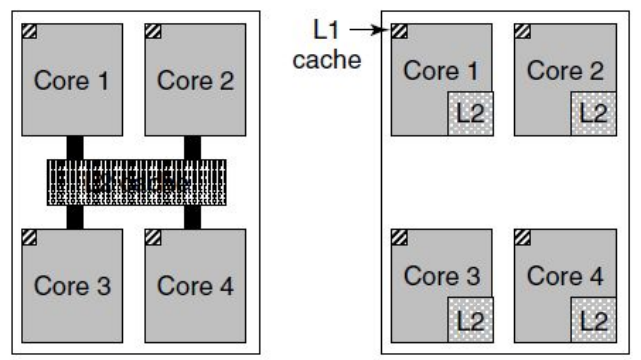
\includegraphics[width=\linewidth]{cpu_caches.png}
\end{theorem}

\begin{definition}{Memory}
    The memory system is constructed as a hierarchy of layers, according to access time:

    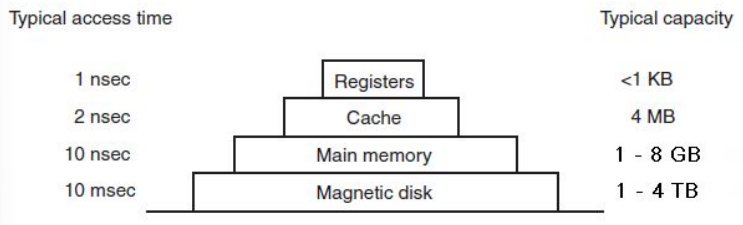
\includegraphics[width=\linewidth]{hardware_review_memory.png}
\end{definition}

\begin{concept}{Input/Output}
    Huge amount of I/O Devices, Hard Drives, Network Interfaces, Serial Ports,
    Keyboard, Mouse, Graphics, Cameras, etc
    \vspace{2mm}\\
    Devices connected with CPU via a Bus System (SW), I/O Interfaces (SW) and I/O
    Controllers (HW)
    \vspace{2mm}\\
    Software that talks to the I/O Controller (Commands/Responses), called Device Driver
    Runs in Kernel or User Mode.
    Built-into Kernel or modular and loadable at boot-/run-time

    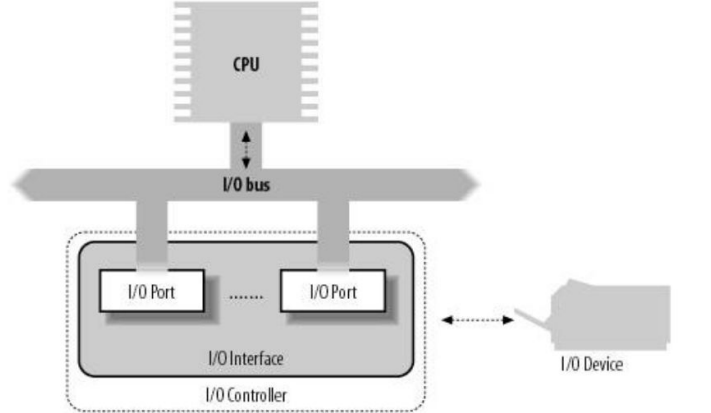
\includegraphics[width=\linewidth]{io_overview.png}
\end{concept}

\begin{example2}{IO and Bus System} X86 System with different Bus standards:

    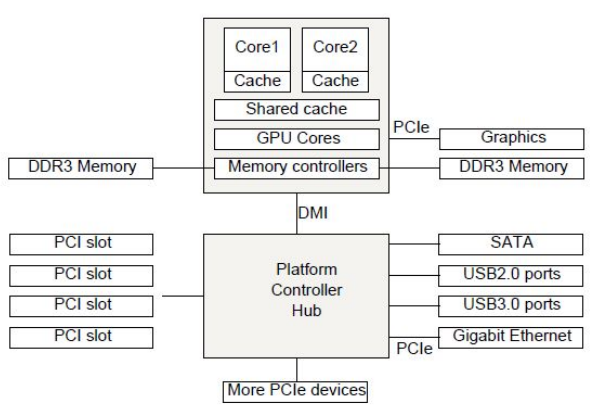
\includegraphics[width=\linewidth]{io_and_bus_syste_example.png}
\end{example2}

\begin{theorem}{Operating System Variants}
    \begin{itemize}
        \item Mainframe OS: IBM z/OS, IBM z/VM
        \item Server OS: Windows Server, Linux, Solaris
        \item Multiprocessor OS: Windows, Linux, Solaris
        \item Personal Computer OS: Windows, MacOS, Linux
        \item Handheld Computer OS: Android, iOS
        \item Embedded OS: VxWorks, QNX
        \item Real-Time OS: VxWorks, QNX
        \item Sensor Node OS: TinyOS, Contiki
        \item Cloud OS: OpenStack, OpenNebula
        \item Smart Card OS: JavaCard, MULTOS
    \end{itemize}
\end{theorem}

\begin{corollary}{Operating Systems vs. Distributions}
    \begin{itemize}
        \item Operating System: Kernel, System Libraries, System Utilities
        \item Distribution: OS + Applications, Tools, Documentation, etc.
    \end{itemize}
    Example: Linux Kernel + GNU Tools + X11 + Gnome + Firefox + LibreOffice = Ubuntu
    \textcolor{pink} evtl. add more info from slides
\end{corollary}

\subsection{Operation System Concepts}

\begin{concept}{Basics}\\
    Interacting with the OS:
    \begin{itemize}
        \item 
    \end{itemize}
    
\end{concept}